\section{Background}
In preparation for my Major Project extensive research was undertaken into the Fuzzy Entropy alignment metrics that would be chosen and implemented in the Congealing algorithm to align mammography scans. S. Al-sharhan's paper `Fuzzy Entropy: a Brief Survey' \cite{Al-Sharhan_Karray_Gueaieb_Basir_2001} was instrumental in a brief comparison between Fuzzy Entropy metrics - allowing a simple way to compare and contrast mathematical differences and implementations.

Researchers have implemented many variations of the Congealing algorithm, with success in varying areas - however very little to no work has been done implementing the algorithm to assess mammography scans. Cox's `Least Squares Congealing' \cite{Cox_Sridharan_Lucey_Cohn_2008} was quickly disregarded given the project preference to select entropy-based alignment techniques, however did alert to the issue of performance for the project.

The motivation behind choosing mammograms as the input data of choice was an interest into how computer systems and machine learning can help in the medical sector - especially in the early diagnosis and/or preventative means of breast cancer. In Europe, breast cancer is the leading cause of death through cancer for women, with 1 in 6 women dying from a cancer having it in the glandular breast tissue \cite{European Commission_2009}. The UK is contained within the higher mortality band which runs across the EU, sitting alongside countries such as the Netherlands, North-West France and Western Germany \ref{fig:mortality-band}. However the reason behind why these countries have a higher breast cancer mortality rate than their neighbours to the north and south is unknown.

\begin{figure}[!ht]
  \center
  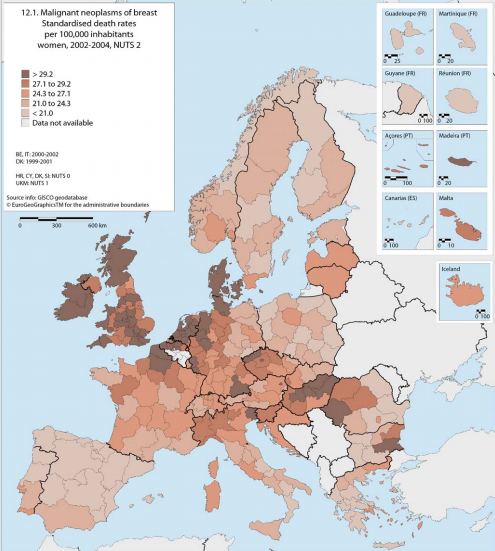
\includegraphics[scale=0.5]{/Users/lauracollins/Git/Major-Project/Documentation/Final/Chapter1/background-img/mortality_EU_Comms.png}
  \caption{Image Source: EU Commission: Atlas on Mortality \cite{European_Commission_2009}}
  \label{fig:mortality-band}
\end{figure}

\subsection{Mammograms}

Quite simply, a Mammogram is an X-Ray of the breast tissue from up to 4 different angles \cite{Radswiki} \cite{Mammography_views_Doc_2016}:
\begin{itemize}
  \item Cranial-Caudal (CC) - taken from above (Figure \ref{fig:CC})
  \item Medio-Lateral Oblique (MLO) - from the side, at an angle (usually 45$/deg$) (Figure \ref{fig:MLO})
  \item Medio-Lateral (ML) - from the centre outwards (Figure \ref{fig:ML})
  \item Latero-Medial (LM) - from the side, into the centre (Figure \ref{fig:LM})
\end{itemize}

CC and MLO are generally the standard practice angles, with ML and LM adding more information for the radiographer to assess.

\begin{figure}[!ht]
  \center
  \begin{subfigure}[ht!]{0.4\textwidth}
        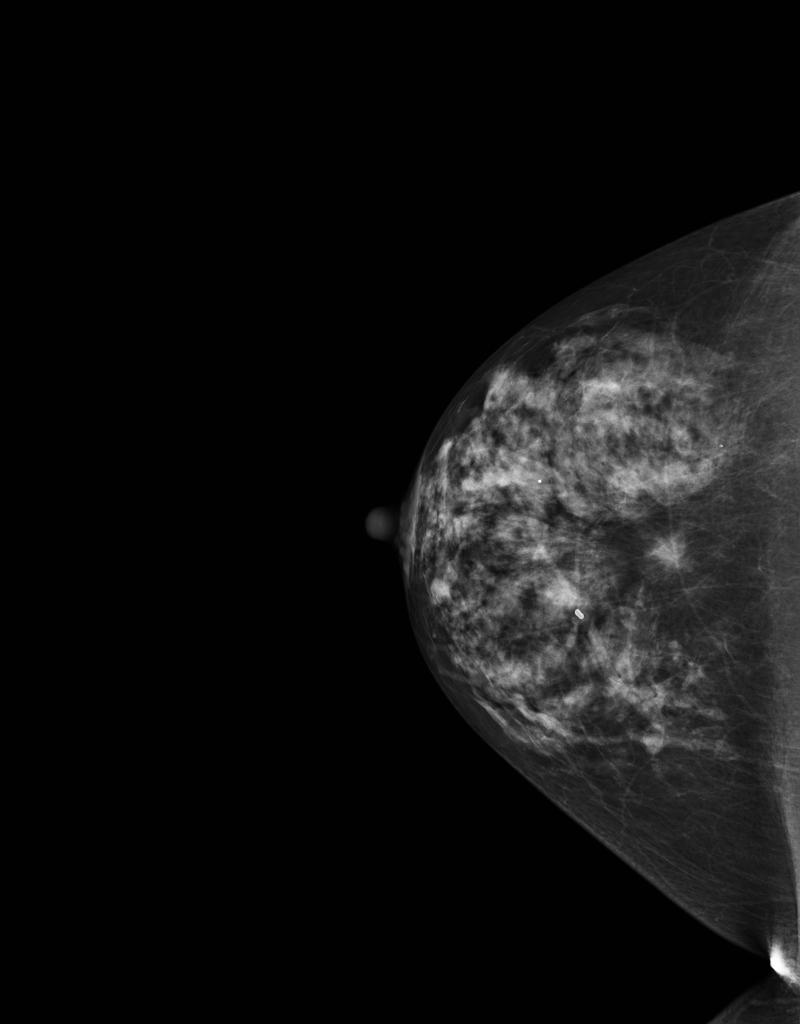
\includegraphics[width=0.5\textwidth]{/Users/lauracollins/Git/Major-Project/Documentation/Final/Chapter1/background-img/CC.jpg}
        \caption{Cranial-Caudal: Case courtesy of Dr Garth Kruger, Radiopaedia.org, rID: 18580}
        \label{fig:CC}
    \end{subfigure}
    \hspace{\fill}
    \begin{subfigure}[ht!]{0.4\textwidth}
          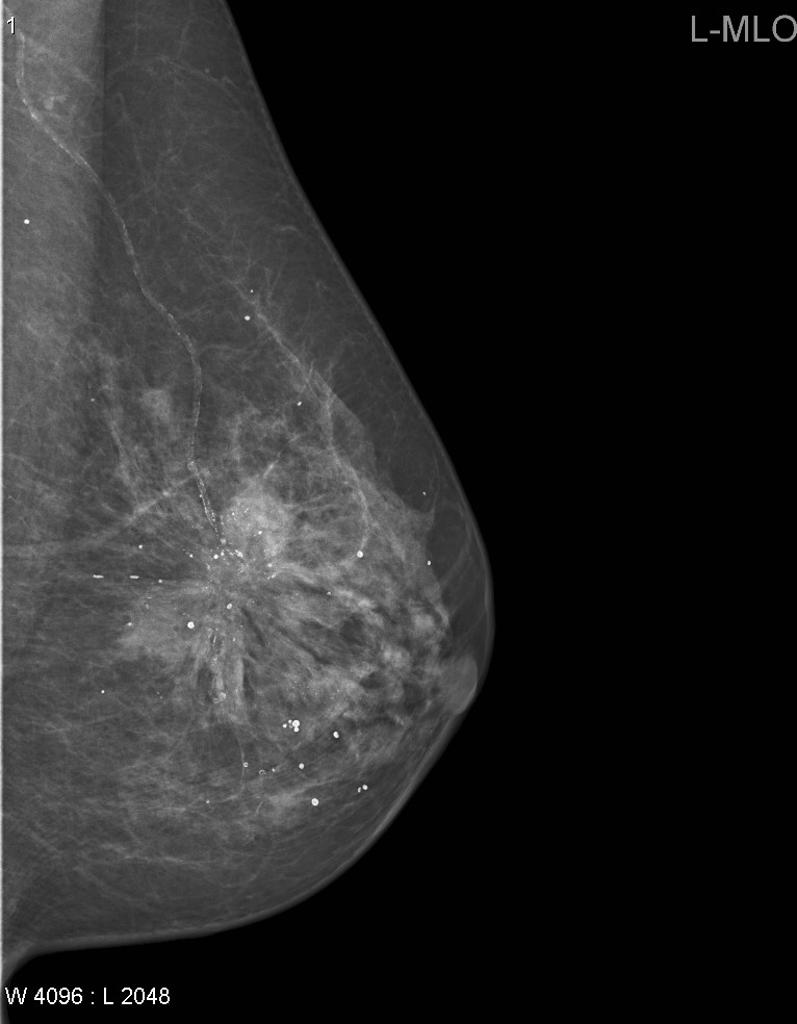
\includegraphics[width=0.5\textwidth]{/Users/lauracollins/Git/Major-Project/Documentation/Final/Chapter1/background-img/MLO.jpg}
          \caption{Medio-Lateral Oblique: Case courtesy of A.Prof Frank Gaillard, Radiopaedia.org, rID: 12608}
          \label{fig:MLO}
    \end{subfigure}

    \begin{subfigure}[ht!]{0.4\textwidth}
          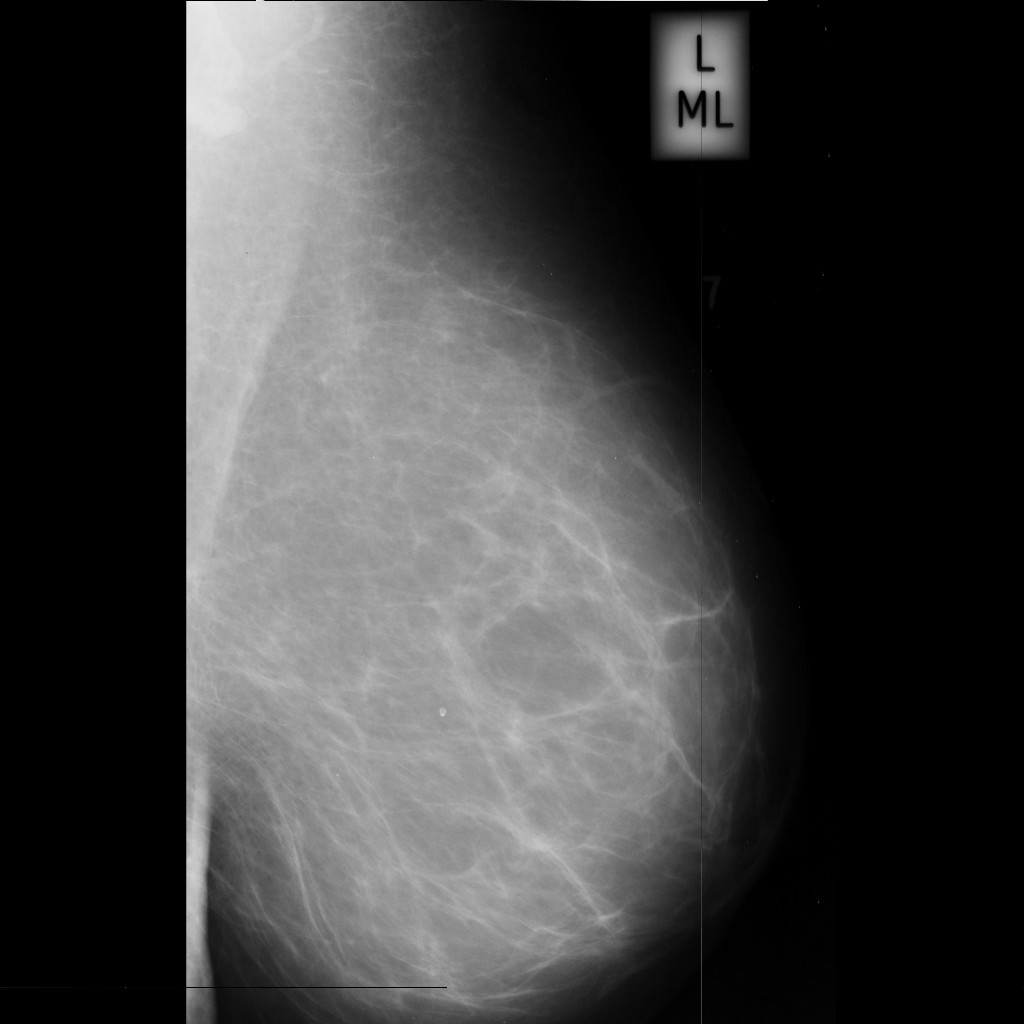
\includegraphics[width=0.5\textwidth]{/Users/lauracollins/Git/Major-Project/Documentation/Final/Chapter1/background-img/ML.jpg}
          \caption{Medio-Lateral: Case courtesy of Mini-MIAS dataset \cite{Suckling_1994}}
          \label{fig:LM}
    \end{subfigure}
    \hspace{\fill}
    \begin{subfigure}[ht!]{0.4\textwidth}
          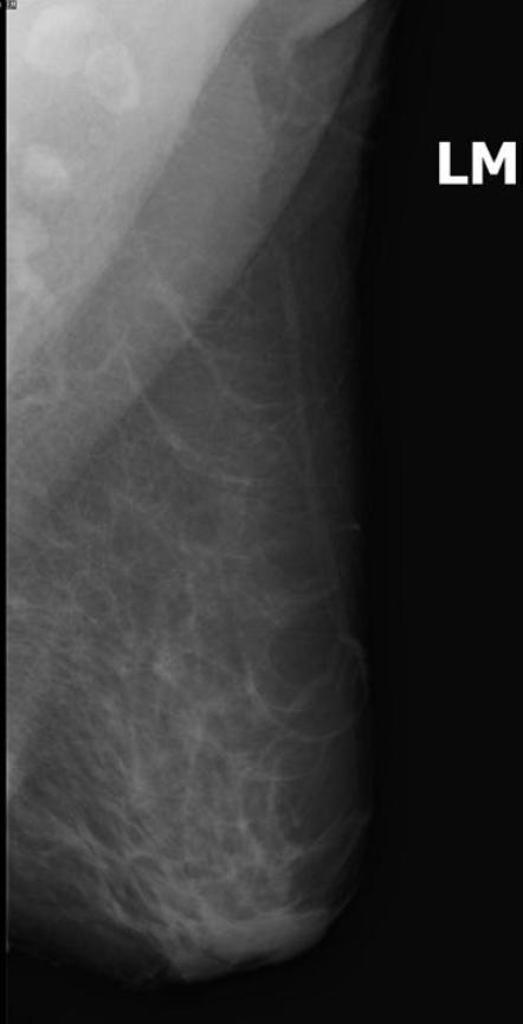
\includegraphics[height=5cm]{/Users/lauracollins/Git/Major-Project/Documentation/Final/Chapter1/background-img/LM.jpg}
          \caption{Latero-Medial: Case courtesy of Dr Paresh K Desai , Radiopaedia.org, rID: 5873}
          \label{fig:ML}
    \end{subfigure}
  \caption{Comparison of the 4 mammogram angles typically used}
  \label{fig:scan-angles}
\end{figure}

Organisations such as Breast Test Wales invite women between the ages of 50 and 70 to attend a scan every 3 years \cite{Informed_Choice_about_Cancer_Screening_2013}. However women with higher-density breasts, which is ascertained during a mammogram, could be called back for more regular screening, to ensure to catch any abnormalities sooner.

\begin{figure}[!ht]
  \center
  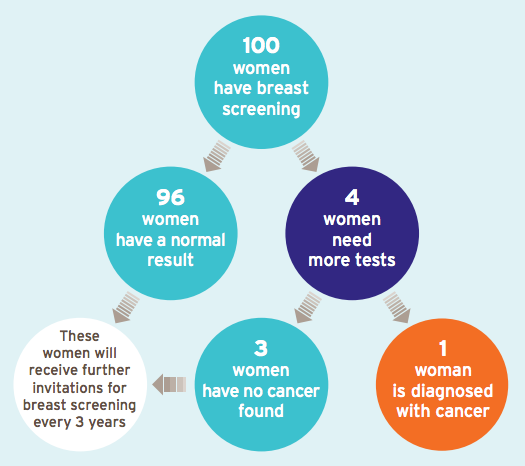
\includegraphics[scale=0.5]{/Users/lauracollins/Git/Major-Project/Documentation/Final/Chapter1/background-img/mammo-leaflet.png}
  \caption{Each time 100 women have breast screening. Image Source: NHS Cancer Screening Programmes \cite{Informed_Choice_about_Cancer_Screening_2013}}
  \label{fig:mammo-leaflet}
\end{figure}

Other breast cancer scanning methods include Ultrasound and a Needle Biopsy. Women under 35 are often offered an ultrasound scan over a mammogram, due to their breasts being of a higher density naturally. Ultrasounds can also show the if the breast lump is a cyst, or if it is solid internally \cite{Cancer_Research_UK_2015}.

\subsection{Tissue density classification}



\subsection{Use of Computer Vision techniques in Medical diagnosis}
